\documentclass[11pt,a4paper]{article}

\usepackage[margin=1.05in]{geometry}
\usepackage{amsmath,amssymb,amsthm}
\usepackage{mathtools}
\usepackage{booktabs}
\usepackage{array}
\usepackage{enumitem}
\usepackage{tikz}
\usetikzlibrary{arrows.meta,positioning,fit,calc}
\usepackage{listings}
\usepackage{xcolor}
\usepackage[T1]{fontenc}
\usepackage[protrusion=true,expansion=false]{microtype}
\usepackage[colorlinks=true,linkcolor=black,citecolor=black,urlcolor=blue]{hyperref}
\setlength{\emergencystretch}{2.5em}
\newcolumntype{L}[1]{>{\raggedright\arraybackslash}p{#1}}

\theoremstyle{plain}
\newtheorem{theorem}{Theorem}[section]
\newtheorem{proposition}[theorem]{Proposition}
\newtheorem{lemma}[theorem]{Lemma}
\newtheorem{corollary}[theorem]{Corollary}
\newtheorem{conjecture}[theorem]{Conjecture}

\theoremstyle{definition}
\newtheorem{definition}[theorem]{Definition}
\newtheorem{example}[theorem]{Example}
\newtheorem{principle}[theorem]{Principle}
\newtheorem{obligation}[theorem]{Obligation}
\newtheorem{finding}[theorem]{Empirical finding}

\theoremstyle{remark}
\newtheorem{remark}[theorem]{Remark}

%%%%%%%%%%%%%%%%%%%%%%%%%%%%%%%%%%%%%%%%%%%%%%%%%%%%%%%%%%%%%%%%%%%%%%%%%%%%%%%
% NOTATION RULES OBSERVED THROUGHOUT:
%   * the rho calculus is never written with the Greek letter rho
%   * quoting is @P, dropping is *x; corner quotes are pre-2016 notation
%%%%%%%%%%%%%%%%%%%%%%%%%%%%%%%%%%%%%%%%%%%%%%%%%%%%%%%%%%%%%%%%%%%%%%%%%%%%%%%
\newcommand{\rhoc}{\textsf{rho}}
\newcommand{\quo}[1]{@#1}
\newcommand{\drp}[1]{{*}#1}
\newcommand{\nil}{\mathbf{0}}
\newcommand{\red}{\longrightarrow}
\newcommand{\wred}{\longrightarrow^{*}}
\newcommand{\nequiv}{\equiv_{\mathcal{N}}}
\newcommand{\scong}{\equiv}
\newcommand{\cmp}[1]{\lfloor #1 \rfloor}
\newcommand{\nms}[1]{\mathcal{N}^{*}(#1)}

\newcommand{\mm}{\mathsf{m}}
\newcommand{\dd}{\mathsf{d}}
\newcommand{\kk}{\mathsf{k}}
\newcommand{\fw}{\mathsf{fw}}
\newcommand{\bl}{\mathsf{b}_{\mathsf{l}}}
\newcommand{\br}{\mathsf{b}_{\mathsf{r}}}
\newcommand{\sy}{\mathsf{s}}
\newcommand{\ev}{\mathsf{e}}
\newcommand{\qq}{\mathsf{q}}
\newcommand{\cons}{\mathsf{cons}}
\newcommand{\consm}{\mathsf{cons}_{\mm}}
\newcommand{\consd}{\mathsf{cons}_{\dd}}
\newcommand{\conss}{\mathsf{cons}_{\sy}}
\newcommand{\consp}{\mathsf{cons}_{\mid}}

\newcommand{\Spec}{\mathcal{S}}
\newcommand{\Nm}{\mathcal{N}}
\newcommand{\Fock}{\mathbb{F}}
\newcommand{\cre}[1]{a^{\dagger}_{#1}}
\newcommand{\ann}[1]{a_{#1}}

\lstdefinestyle{py}{
  basicstyle=\footnotesize\ttfamily, breaklines=true,
  keywordstyle=\color{blue!60!black}, commentstyle=\color{green!40!black},
  showstringspaces=false, frame=single, framerule=0.3pt,
  rulecolor=\color{black!35}, columns=flexible,
}

\title{\textbf{Rho Combinators as Sparse Linear Algebra}\\[4pt]
\large A classical route from reflective concurrency to data-parallel execution}
\author{L.\,G.\ Meredith\\
\small CEO, F1R3FLY.io, and Chief Science Officer, F1R3FLY Industries}
\date{22 September 2026 --- version 1}

\begin{document}
\maketitle

\begin{abstract}
\noindent
The question this note answers is whether the concurrency of the \rhoc{}
calculus can be mapped onto the concurrency of a graphics processor by way of
the name-free combinators, and specifically whether the reduction graph of a
combinator term admits a matrix representation that factors into a
representation of the rewrite rules and repeated application to a vector
encoding of a term. The scope here is strictly classical: no weights, no
amplitudes, no quantum reading.

The answer has three parts. First, the factorisation exists and is standard,
once the right state space is identified. The companion logic note proves
that the multiset of top-level atoms is a complete invariant for structural
congruence, so a combinator state \emph{is} an occupation vector and the one-step
operator is a sum of ladder-operator monomials, one per rule, each of degree
at most four. The equations of the calculus are quotiented by construction
rather than by normalisation.

Second, the three invariants used in the draft's expressiveness lattice ---
name closure, atom count, message count --- turn out to be exactly the three
finiteness conditions the matrix representation requires, and each is
controlled by a different axis of the lattice. Name closure controls the index
set, so the constructors decide whether the basis is finite or generated on
demand. Atom count controls nilpotency, so the destructor decides whether the
transfer operator is strictly block upper triangular. Message count controls
occupation bounds. The lattice therefore already computes which matrix shape a
term admits, and the eager and lazy parts of the operator are separated by the
same analysis: seven of the twelve rules are constant-coefficient and fully
schematic, four require an encode, and exactly one, the destructor, requires a
decode.

Third, and this is the practical finding, the object worth multiplying is not
the transition matrix of the reduction graph. It is the incidence matrix of
atoms against names, which is term-sized and sparse. Redex finding for every
rule is a join on that matrix, conflict detection between redexes is a second
sparse product, and a machine step is a maximal independent set in the
resulting conflict graph. Firing an independent set is sound with respect to
the interleaving semantics, so the number of machine steps is the causal
depth of the computation rather than its interleaving length. That ratio is
the available speedup, and it is measurable. A reference implementation
accompanies the note; its matrix formulation of redex finding agrees with
naive enumeration on 400 random states, and on four families of terms the
measured ratio of sequential steps to parallel steps is exactly the width of
the term.

A phased development plan and seven numbered obligations close the note.
\end{abstract}

\tableofcontents

%==============================================================================
\section{What this note is}
\label{sec:what}

This note is a design analysis, not a completed theory. It records what the
rho combinators of the draft in \texttt{F1R3FLY-io/publications/rho-combinators}
already give a machine builder, what they do not, and in what order the
remaining work should be attempted.

\paragraph{Scope.} Classical execution only. Everything here is over the
Boolean semiring or the natural numbers. The weighted, complex-valued and
quantum readings developed elsewhere in the programme are deliberately absent;
they attach to the same operator later, as \S\ref{sec:notdo} notes, and
nothing below depends on them.

\paragraph{Claims.} Six, and nothing more.
\begin{enumerate}[label=(C\arabic*),leftmargin=3em]
\item A combinator state is an occupation vector over a species set, with
  structural congruence quotiented by construction
  (\S\ref{sec:states}).
\item The one-step relation is a sum of twelve ladder-operator monomials of
  degree at most four, schematic in the names (\S\ref{sec:operator}).
\item The three invariants of the draft's lattice section are the three
  finiteness conditions of that operator, one per lattice axis
  (\S\ref{sec:three}).
\item Upper triangularity holds exactly on the destructor-free fragment, and
  the general case needs either the history unfolding or nothing at all
  (\S\ref{sec:triangular}).
\item Redex finding and conflict detection are sparse matrix products on the
  atom-name incidence matrix, which is term-sized (\S\ref{sec:multiply}).
\item Firing a maximal independent set of redexes per step is sound with
  respect to the interleaving semantics, so machine steps count causal depth
  (\S\ref{sec:step}).
\end{enumerate}

\paragraph{Not claimed.} That any of this beats a well-tuned sequential
interpreter on real workloads; the measurements in \S\ref{sec:measure} are on
synthetic term families chosen to exhibit known widths, and the width of
compiled \rhoc{} programs is unmeasured. That the reduction graph itself
should ever be materialised; the position taken here is the opposite. That
maximal progress is the right resolver; it is \emph{a} resolver, and
Obligation~\ref{obl:resolver} asks what it costs.

\paragraph{Status markers.} \textsf{SETTLED} for what is proved or measured
here or cited from the companion drafts; \textsf{ROUTE} for a construction
believed to work whose details are not discharged; \textsf{OPEN} for a
question with no proposed answer; \textsf{GATE} for something that must be
settled before the work downstream of it is worth starting.

%==============================================================================
\section{The two machines}
\label{sec:machines}

The mapping asked for is between two concurrency paradigms, so it is worth
writing down what each actually is before looking for a morphism.

\subsection{What a graphics processor rewards}

A modern accelerator is a bulk-synchronous machine with a very wide, very
shallow execution model. It rewards, in rough order of importance:

\begin{enumerate}[label=(G\arabic*),leftmargin=3em]
\item \textbf{Flat, indexable state.} Arrays of fixed-width records at
  predictable addresses. Pointer chasing through a heap of variably shaped
  nodes is the single most expensive thing one can ask of it.
\item \textbf{Uniform work across lanes.} Threads in a warp that take the same
  branch. Data-dependent control flow serialises.
\item \textbf{Bulk-synchronous phases.} A kernel launch does one thing to
  everything, then a barrier. Fine-grained locking and point-to-point
  synchronisation between work items are not available cheaply.
\item \textbf{Standard sparse primitives.} Sparse matrix--vector and
  matrix--matrix products, segmented scans, sorts, and hash tables have
  mature, heavily optimised implementations. Work expressed in those terms
  inherits decades of tuning; work expressed otherwise does not.
\end{enumerate}

\subsection{What a tuple-space interpreter does}

An RSpace-style interpreter for the \rhoc{} calculus does approximately the
opposite of all four. Its state is a store of variably shaped terms reached by
pointer; matching a receipt against a datum is a recursive walk over nested
syntax with binder-sensitive pattern variables; conflicts between competing
comm events are resolved by locking or by a single-threaded scheduler; and the
inner loop is a hash lookup followed by unification, which is not a sparse
linear algebra primitive by any reading.

None of that is a criticism of RSpace, which is a good design for a general
machine. It is an observation that the gap between the two paradigms is
concrete and itemised, and that a compiler standing between them has a
specific job description.

\subsection{The gap, and who closes it}

The combinators close three of the four gaps by themselves, and the fourth is
closed by the step semantics of \S\ref{sec:step}.

\begin{center}
\begin{tabular}{@{}L{0.31\textwidth}L{0.60\textwidth}@{}}
\toprule
\textbf{Accelerator wants} & \textbf{What supplies it} \\
\midrule
(G1) flat indexable state &
  Combinator atoms are fixed-arity tuples of names; under presentation~A every
  argument is a name, hence an integer index (\S\ref{sec:facts}). \\
(G2) uniform work &
  Twelve rules, each a fixed shape; one kernel per rule, no pattern matching
  at runtime. The pattern matching happened in the compiler. \\
(G3) bulk-synchronous phases &
  A step fires a maximal independent set of redexes, which is one barrier per
  causal layer (\S\ref{sec:step}). \\
(G4) sparse primitives &
  Redex finding is a join, conflict detection is a product, independent-set
  selection is a standard parallel primitive (\S\ref{sec:multiply}). \\
\bottomrule
\end{tabular}
\end{center}

The compiler from the \rhoc{} calculus to the combinators is therefore
load-bearing rather than decorative: it is the component that moves pattern
matching from run time to compile time, and it costs only a constant factor in
term size (draft 3, Prop.~8.1: the image has $O(|P|)$ atoms).

%==============================================================================
\section{The combinators, and four structural facts}
\label{sec:facts}

The calculus is that of draft~3, in the repaired form: two sorts, atoms
\[
\mm,\ \dd,\ \kk,\ \fw,\ \bl,\ \br,\ \sy,\ \ev,\ \qq,\ \consp,\ \consm,
\ \consd,\ \conss,
\]
the equations of an abelian monoid on $\mid$ together with
$\quo{\drp{a}} = a$, and, under presentation~A, $\drp{\quo{p}} = p$. The
twelve rewrite rules are reproduced in Figure~\ref{fig:rules}.

\begin{figure}[t]
\hrule\vspace{4pt}
\[
\begin{array}{l@{\qquad}l}
 \dd(a,b,c) \mid \mm(a,v) \red \mm(b,v) \mid \mm(c,v)
   & \bl(a,b) \mid \mm(a,v) \red \fw(v,b)\\
 \kk(a) \mid \mm(a,v) \red \nil
   & \br(a,b) \mid \mm(a,v) \red \fw(b,v)\\
 \fw(a,b) \mid \mm(a,v) \red \mm(b,v)
   & \sy(a,b,c) \mid \mm(a,v) \red \fw(b,c)\\
 \ev(a) \mid \mm(a,v) \red \drp{v}
   & \fw(a,b) \mid \qq(a,p) \red \mm(b,\quo{p})\\[4pt]
 \multicolumn{2}{l}{\consp(a,b,c) \mid \mm(a,\quo{p}) \mid \mm(b,\quo{r})
   \red \mm(c,\quo{(p \mid r)})}\\
 \multicolumn{2}{l}{\consm(a,b,c) \mid \mm(a,u) \mid \mm(b,v)
   \red \mm(c,\quo{\mm(u,v)})}\\
 \multicolumn{2}{l}{\consd(a,b,c,f) \mid \mm(a,u) \mid \mm(b,v) \mid \mm(c,w)
   \red \mm(f,\quo{\dd(u,v,w)})}\\
 \multicolumn{2}{l}{\conss(a,b,c,f) \mid \mm(a,u) \mid \mm(b,v) \mid \mm(c,w)
   \red \mm(f,\quo{\sy(u,v,w)})}
\end{array}
\]
\vspace{2pt}\hrule
\caption{The twelve rules, closed under $\mid$ and under the equations, with
subjects matched up to $\nequiv$.}
\label{fig:rules}
\end{figure}

Four facts about this presentation do the work of the rest of the note. Three
are theorems of the companion drafts; the fourth is a design recommendation.

\begin{enumerate}[label=(F\arabic*),leftmargin=3em]
\item \textbf{Atoms are flat.} Every atom is a head symbol applied to at most
  four arguments, and every argument is a name, except the payload of $\qq$
  and, under presentation~B, of $\mm$. There is no nesting, no binder, and no
  pattern variable.
\item \textbf{The multiset is complete.} By the logic note's component lemma,
  $\cmp{P}$, the multiset of top-level atoms of the drop-free normal form, is
  a complete invariant: $P \scong Q$ iff $\cmp{P} = \cmp{Q}$ as multisets.
  \textsf{SETTLED}
\item \textbf{Rules are small and subject-joined.} Every rule has between two
  and four premises, each premise a single atom, and the premises share names.
  The logic note remarks that this is the only structural fact its modality
  uses; it is also the only structural fact the machine below uses.
  \textsf{SETTLED}
\item \textbf{Name equality is decidable and internable.} On closed drop-free
  normal forms $\nequiv$ is decidable, by normalisation followed by multiset
  comparison, and $\quo{-}$ is injective there. So names can be hash-consed to
  integers once and compared by integer equality thereafter. \textsf{SETTLED}
\end{enumerate}

\begin{remark}[Presentation A is the machine presentation]
\label{rem:AforA}
Draft~3 leaves the choice between presentations A and B open on grounds of
where decoding happens. For a machine the choice is forced, and in favour
of~A. Under~A a message payload is a name, hence an integer, so every atom is
a fixed-width tuple of integers and (G1) is satisfied exactly. Under~B a
payload is a process, so an atom is a tuple of integers together with a
variable-sized block, and the store becomes ragged.

The same move should be made for $\qq$. Although its payload is sorted as a
process, storing it by its quote --- holding $\qq(a,p)$ as the pair
$(a, \quo{p})$ --- loses nothing, because $\quo{-}$ is injective on normal
forms by (F4), and it makes the $\mathsf{quote}$ rule a field copy rather than
a construction. This is the difference between rule class (a) and class (b) in
\S\ref{sec:operator}, and it is obtained for free. \textsf{SETTLED}
\end{remark}

%==============================================================================
\section{States are occupation vectors}
\label{sec:states}

\begin{definition}[Species]
\label{def:species}
A \emph{species} is a pair of a head symbol and a tuple of names of the
matching arity: the set is
$\Spec = \{ (A, \vec{n}) : A \text{ a head symbol}, \vec{n} \in
\Nm^{\mathrm{ar}(A)} \}$, where $\Nm$ is the set of names modulo $\nequiv$.
\end{definition}

By (F2) a state is a finite multiset over $\Spec$, that is, a function
$\gamma : \Spec \to \mathbb{N}$ of finite support. Write $\Fock$ for the free
module on the set of such $\gamma$ and $|\gamma\rangle$ for the basis vector
at $\gamma$. Equivalently, and more usefully, $\Fock$ is the free commutative
algebra generated by $\Spec$: a state is a monomial
$\prod_{\sigma} (\cre{\sigma})^{\gamma(\sigma)}\,|\nil\rangle$, and the abelian
monoid equations of the calculus are the commutativity of that product.

\begin{principle}[Structural congruence is free]
\label{prin:free}
The equations of Definition~3.2 of draft~3 are not imposed on the
representation and are not discharged by a normalisation pass. Commutativity,
associativity and the unit of $\mid$ are the algebra of the multiset;
$\drp{\quo{p}} = p$ and $\quo{\drp{a}} = a$ are discharged once, at
interning time, by the drop-elimination lemma. No run-time cost. \textsf{SETTLED}
\end{principle}

This is the first place where the combinators pay. In a direct \rhoc{}
machine, matching modulo structural congruence is a recurring cost and a
recurring source of subtlety; here it is a property of the data structure.

\subsection{Names, and the self-indexing problem}

$\Spec$ is indexed by $\Nm$, and $\Nm$ is the set of quoted processes, so by
(F2) it is the set of finite multisets over $\Spec$. The index set of the
basis therefore satisfies
\[
  \Nm \;\cong\; M_{\mathrm{fin}}(\Spec), \qquad
  \Spec \;=\; \textstyle\coprod_{A} \Nm^{\mathrm{ar}(A)} .
\]
The basis of the state space indexes itself. This is reflection, seen through
the linear algebra, and it is the reason no finite matrix can be written down
in advance for the full calculus. The solution of the domain equation is the
initial algebra: names are finite trees, so $\Nm$ is countable, finitely
branching, and graded by depth of quotation.

\begin{definition}[The intern table]
\label{def:intern}
The machine realises $\Nm$ as a bijection between integers and canonical
component multisets, in two directions:
\[
\begin{array}{ll}
  \mathsf{quote} : M_{\mathrm{fin}}(\Spec) \to \mathbb{N}
    & \text{hash-cons; an encode,}\\[2pt]
  \mathsf{drop} : \mathbb{N} \to M_{\mathrm{fin}}(\Spec)
    & \text{table read; a decode.}
\end{array}
\]
\end{definition}

\begin{remark}[Interning order is a gauge freedom]
\label{rem:gauge}
Two runs that fire the same rules in different orders may assign different
integers to the same name, because integers are handed out on insertion. The
resulting states are equal up to the canonical bijection determined by
$\mathsf{quote}$, which is injective. Nothing observable depends on the
assignment, and the machine must never let an integer comparison stand in for
a semantic distinction between runs. \textsf{SETTLED}
\end{remark}

%==============================================================================
\section{The rule operator}
\label{sec:operator}

\begin{definition}[Ladder operators]
For $\sigma \in \Spec$, let $\cre{\sigma}$ add one occurrence of $\sigma$ and
$\ann{\sigma}$ remove one, with $\ann{\sigma}|\gamma\rangle = 0$ when
$\gamma(\sigma) = 0$.
\end{definition}

\begin{definition}[The transfer operator]
\label{def:T}
For a rule $r$ with premise multiset $L_r$ and conclusion multiset $R_r$, both
over atom shapes with name variables, and for a substitution $\theta$ of those
variables by names,
\[
  H_r \;=\; \sum_{\theta}
  \Bigl(\prod_{\beta \in R_r\theta} \cre{\beta}\Bigr)
  \Bigl(\prod_{\alpha \in L_r\theta} \ann{\alpha}\Bigr),
  \qquad
  T \;=\; \sum_{r} H_r .
\]
\end{definition}

This is the factorisation asked for. $T$ is a representation of the rewrite
rules alone: it is schematic in the names, independent of any particular term,
and of degree at most four by (F3). The unfolding of the reduction graph is
repeated application of $T$ to $|\gamma\rangle$.

\begin{proposition}[Matrix elements count derivations]
\label{prop:counts}
$\langle \gamma' | H_r | \gamma\rangle$ is the number of distinct occurrence
tuples in $\gamma$ matching $L_r$ and producing $\gamma'$, namely
$\prod_{\alpha} (\gamma(\alpha))_{\underline{m_\alpha}}/\prod_\alpha
m_\alpha!$ where $m_\alpha$ is the multiplicity of $\alpha$ in $L_r\theta$ and
$(n)_{\underline{m}}$ is the falling factorial.
\end{proposition}

\begin{proof}
Standard for multiset rewriting: a match is a choice of $m_\alpha$ distinct
occurrences of each premise species, unordered within a species.
\end{proof}

\begin{remark}[This is mass action, and it is not an accident]
Proposition~\ref{prop:counts} is the mass-action law, and the coefficient is
the same multiplicity $h$ that the Gillespie implementation in
\texttt{rho-life} already computes. The combinators are a chemical reaction
network with twelve reaction schemes. The classical reading taken here uses
only the Boolean shadow of that coefficient; the weighted readings elsewhere
in the programme use the coefficient itself.
\end{remark}

\subsection{Three classes of rule}
\label{sec:classes}

The twelve rules are not alike in how much of $T$ can be written down ahead of
time.

\begin{description}[leftmargin=2.2em,style=nextline]
\item[Class (a), seven rules: permutation of existing indices.]
  $\mathsf{dist}$, $\mathsf{kill}$, $\mathsf{forward}$, $\mathsf{bind_l}$,
  $\mathsf{bind_r}$, $\mathsf{synch}$, $\mathsf{quote}$. The conclusion is a
  fixed multiset of atoms whose names all occur in the premise. $H_r$ is a
  constant-coefficient ladder monomial, fully schematic, requiring no access
  to the intern table at all. Note that $\mathsf{quote}$ belongs here only
  because of Remark~\ref{rem:AforA}.
\item[Class (b), four rules: encode.] The four constructors. The conclusion is
  a single atom, so the arity is fixed, but its payload is a \emph{new} index,
  obtained by hash-consing a term built from the premise names. $H_r$ grows
  the index set.
\item[Class (c), one rule: decode.] $\mathsf{eval}$. It is the only rule whose
  conclusion multiset has a size depending on the \emph{value} of a premise
  name. Its rows cannot be written schematically; they require reading the
  intern table.
\end{description}

\begin{principle}[Where the laziness is, and which kind]
\label{prin:lazy}
The matrix must be materialised lazily for two distinct reasons, and the
lattice separates them. Class (b) makes the \emph{basis} generate on demand:
new columns appear. Class (c) makes the \emph{rows} generate on demand: an
existing column's image is not known until the index is decoded. Class (a),
which is most of the calculus, is fully eager. \textsf{SETTLED}
\end{principle}

%==============================================================================
\section{Three invariants, three finiteness conditions}
\label{sec:three}

Section~9 of draft~3 proves three invariants in order to draw the
expressiveness lattice. They are, without modification, the three finiteness
conditions a matrix representation needs, and each is governed by a different
axis of the lattice. This is the note's main structural observation.

\begin{theorem}[The lattice classifies the matrix]
\label{thm:three}
Let $T$ be a combinator term over a constructor set $S$.
\begin{enumerate}[label=(\roman*),leftmargin=2.4em]
\item \emph{(Index set; constructor axis.)} By the name-closure lemma, every
  name occurring in a reduct of $T$ lies in the closure of $\nms{T}$ under the
  node shapes $\{A : \cons_A \in S\}$. If $S = \emptyset$ the reachable name
  set is $\nms{T}$, which is finite, so $\Spec$ restricted to reachable
  species is finite of size $O(|\nms{T}|^{4})$. If $S \neq \emptyset$ the
  reachable name set is the free $S$-algebra on $\nms{T}$, countable and
  graded by depth.
\item \emph{(Nilpotency; destructor axis.)} By the atom-count lemma every rule
  but $\mathsf{eval}$ strictly decreases the number of non-message atoms. Let
  $N$ be that number in $T$. Without $\ev$, the function $\gamma \mapsto
  N(\gamma)$ is a grading strictly decreased by every step, so the reachable
  sub-operator is strictly block upper triangular with respect to it and
  $T^{N+1} = 0$.
\item \emph{(Occupation bound; duplication axis.)} By the message-count lemma
  $\dd$ is the only rule that increases the number of messages without
  consuming a $\qq$ or opening a payload, so without $\dd$ and without $\ev$
  the message count is non-increasing and occupation numbers are bounded by
  those of $T$.
\end{enumerate}
\end{theorem}

\begin{proof}
Each clause is the cited lemma read as a statement about the operator. For
(ii), a strictly decreasing integer grading bounded below by $0$ and above by
$N$ gives a block decomposition in which $T$ maps block $j$ into blocks
$< j$, which is the definition of strict block upper triangularity, and
composition of $N+1$ such maps is zero.
\end{proof}

\begin{corollary}[Closed-form reachability on the destructor-free fragment]
\label{cor:neumann}
Without $\ev$, the reachability closure is the terminating Neumann series
$\sum_{k \le N} T^{k} = (\mathbf{1} - T)^{-1}$, computable in
$\lceil \log_2 N\rceil$ repeated squarings, each a sparse matrix product.
\textsf{SETTLED}
\end{corollary}

\begin{remark}[One atom, three characterisations]
\label{rem:evthrice}
The destructor $\ev$ is, simultaneously: the carrier of Turing power, by the
draft's strong-normalisation proposition; the unique breaker of the grading,
by Theorem~\ref{thm:three}(ii); and the unique rule whose operator cannot be
written schematically, by \S\ref{sec:classes}. Three independent
characterisations of the same atom, arrived at from logic, from order theory
and from implementation. The draft's remark that ``the destructor carries the
computational power that reflection supplies'' acquires an operational
reading: the power is exactly the ability to turn an index into a state.
\end{remark}

\begin{remark}[The Petri net reading]
Without constructors and without $\ev$, the combinators are a
place/transition net: places are species, transitions are rule instances, and
the step semantics of \S\ref{sec:step} is the net's step semantics. Adding
constructors makes the place set generated rather than given; adding $\ev$
makes the transition relation depend on the contents of a place. The lattice
is therefore also a descent from nets through generated-place nets to Turing
completeness, which is a second reading of the same three invariants and may
be worth a paragraph in the draft. \textsf{ROUTE}
\end{remark}

\subsection{Upper triangularity, precisely}
\label{sec:triangular}

The proposal that opened this line of work was to encode the reduction graph
as an upper triangular matrix. Upper triangularity is equivalent to acyclicity
of the graph, and the reduction graph of a combinator term is not acyclic in
general: reflection admits terms that step to a structurally congruent copy of
themselves, and by Principle~\ref{prin:free} structurally congruent means
equal. So on the nose the encoding is available exactly on the
destructor-free fragment, by Theorem~\ref{thm:three}(ii).

Two repairs are available, and for the classical execution goal the second is
recommended.

\begin{enumerate}[label=(\arabic*),leftmargin=2.4em]
\item \textbf{Work in the unfolding.} The free history of a term is the
  universal cover of its reduction graph, graded by step count, hence acyclic
  by construction; triangularity is then free, at the cost of never
  identifying a returning state. The cycles one gives up are exactly the
  non-trivial elements of $\pi_1$ that the history endofunctor's erasure
  lattice already parametrises, so the apparatus exists. This is the right
  route if the closure is the object wanted, for instance for model checking.
  \textsf{ROUTE}
\item \textbf{Do not ask for it.} For running a program one needs a frontier,
  not a closure: the current state and its successors. Triangularity is a
  property of the whole graph and buys nothing at the frontier. A general
  sparse non-negative operator applied to a sparse vector is entirely
  adequate, and iterative methods are indifferent to cycles.
  \textsf{SETTLED}
\end{enumerate}

%==============================================================================
\section{What actually gets multiplied}
\label{sec:multiply}

There are three matrices in play and conflating them is the easiest mistake to
make here.

\begin{center}
\begin{tabular}{@{}llL{0.42\textwidth}@{}}
\toprule
& \textbf{Indexed by} & \textbf{Size, and what it is for} \\
\midrule
$T$ & markings $\times$ markings &
  Astronomically large, never materialised. The semantics. \\
$B$ & redexes $\times$ occurrences &
  $O(\text{redexes})$ nonzeros. Conflict detection. \\
$A$ & atom occurrences $\times$ names &
  \textbf{Term-sized}, exactly $\sum_{\text{atoms}} \mathrm{ar}(A)$ nonzeros.
  The thing the machine multiplies. \\
\bottomrule
\end{tabular}
\end{center}

\begin{definition}[Incidence]
\label{def:inc}
For each head symbol $A$ and each argument slot $j < \mathrm{ar}(A)$, let
$M^{A}_{j}$ be the Boolean matrix with $M^{A}_{j}[i,n] = 1$ iff the $i$-th
occurrence of $A$ carries name $n$ in slot $j$. Each row has exactly one
nonzero; the whole family has $\sum_{\text{atoms}} \mathrm{ar}(A) \le 4|\gamma|$
nonzeros.
\end{definition}

\subsection{Redex finding is a join}

By (F3) every rule is a conjunction of atom premises sharing names, which is a
relational join on the incidence matrices. Writing $\cdot$ for Boolean sparse
matrix product:

\begin{center}\small
\begin{tabular}{@{}L{0.19\textwidth}L{0.33\textwidth}L{0.38\textwidth}@{}}
\toprule
\textbf{Rules} & \textbf{Expression} & \textbf{Cost} \\
\midrule
the seven two-premise rules against $\mm$
  & $M^{C}_{0} \cdot (M^{\mm}_{0})^{\!\top}$
  & one \textsc{SpGEMM}; nonzeros
    $\sum_{n} c_{n}\mu_{n}$ where $c_n,\mu_n$ are the numbers of consumers and
    messages at $n$ \\
$\mathsf{quote}$
  & $M^{\fw}_{0} \cdot (M^{\qq}_{0})^{\!\top}$ & as above \\
$\consp, \consm$
  & $X = M^{\cons}_{0}\cdot(M^{\mm}_{0})^{\!\top}$,
    $Y = M^{\cons}_{1}\cdot(M^{\mm}_{0})^{\!\top}$, then the row-wise
    Cartesian product $X \bowtie Y$ with $j \neq k$ masked out
  & two \textsc{SpGEMM}s plus a segmented expansion \\
$\consd, \conss$
  & three such products, then a three-fold row-wise product with
    distinctness masking
  & three \textsc{SpGEMM}s plus expansion \\
\bottomrule
\end{tabular}
\end{center}

\begin{remark}[Contention is a join cost, not a scheduling cost]
\label{rem:contention}
The two-premise product has $\sum_n c_n \mu_n$ nonzeros, which is quadratic in
the occupancy of a contended channel. This is real and is measured in
\S\ref{sec:measure} (experiment E2, where $c$ consumers and $c$ messages on
one channel produce $c^{2}$ redexes). It does \emph{not} cost parallelism:
the maximal independent set on that quadratic redex set is a perfect matching
of size $c$, found in one step. The cost is enumeration, and the standard
remedy --- worst-case-optimal join, or bucketing by name before the product ---
applies unchanged. \textsf{OPEN} which remedy is right at scale.
\end{remark}

\subsection{Conflict detection is a second product}

\begin{definition}[Conflict]
Two redexes conflict if they consume a common occurrence. With $B$ the
redex-occurrence incidence matrix, the conflict graph is the off-diagonal
nonzero pattern of $B\cdot B^{\top}$.
\end{definition}

So the entire per-step analysis --- which redexes exist, and which of them may
fire together --- is two rounds of Boolean sparse matrix multiplication on
term-sized operands. That is the concrete content of ``\rhoc{} execution as
linear algebra'' in the classical setting, and it involves no matrix whose
dimension is the number of states.

\begin{figure}[t]
\centering
\resizebox{\textwidth}{!}{%
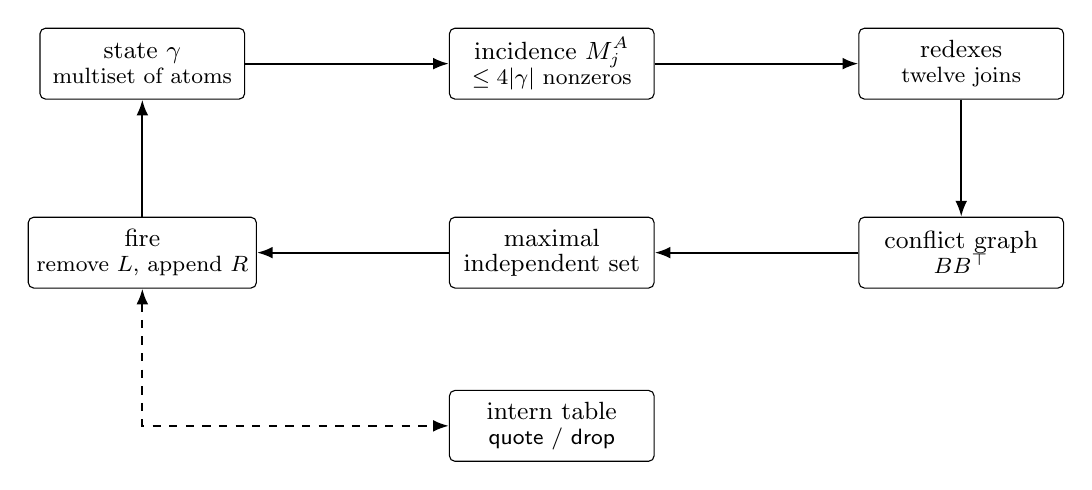
\begin{tikzpicture}[
  box/.style={draw, rounded corners=2pt, align=center, font=\small,
              minimum height=9mm, minimum width=26mm, inner sep=3pt},
  ar/.style={-{Latex[length=2mm]}, thick}]
\node[box] (st)  at (0,0)    {state $\gamma$\\[-2pt] \footnotesize multiset of atoms};
\node[box] (inc) at (5.2,0)  {incidence $M^{A}_{j}$\\[-2pt] \footnotesize $\le 4|\gamma|$ nonzeros};
\node[box] (rdx) at (10.4,0) {redexes\\[-2pt] \footnotesize twelve joins};
\node[box] (cfl) at (10.4,-2.4) {conflict graph\\[-2pt] \footnotesize $BB^{\top}$};
\node[box] (mis) at (5.2,-2.4)  {maximal\\[-2pt] independent set};
\node[box] (fire) at (0,-2.4)   {fire\\[-2pt] \footnotesize remove $L$, append $R$};
\node[box] (tab) at (5.2,-4.6)  {intern table\\[-2pt] \footnotesize $\mathsf{quote}$ / $\mathsf{drop}$};
\draw[ar] (st)  -- (inc);
\draw[ar] (inc) -- (rdx);
\draw[ar] (rdx) -- (cfl);
\draw[ar] (cfl) -- (mis);
\draw[ar] (mis) -- (fire);
\draw[ar] (fire) -- (st);
\draw[{Latex[length=2mm]}-{Latex[length=2mm]},dashed,thick] (fire) |- (tab);
\end{tikzpicture}}
\caption{One machine step. Every solid arrow is a data-parallel bulk
operation. The dashed arrow is the encode and the decode of
\S\ref{sec:reflection}, used only by rule classes (b) and (c).}
\label{fig:step}
\end{figure}

%==============================================================================
\section{The parallel step}
\label{sec:step}

This section supplies (G3), and is where the concurrency of the calculus meets
the concurrency of the machine.

\begin{definition}[Independence, step]
\label{def:step}
Redexes $r_1, r_2$ enabled in $\gamma$ are \emph{independent} if the
occurrence multisets they consume are disjoint. A set $S$ of pairwise
independent redexes is a \emph{step}; $\gamma \Rightarrow_S \gamma'$ removes
every occurrence consumed by a member of $S$ and adds every atom produced by a
member of $S$.
\end{definition}

\begin{lemma}[Diamond]
\label{lem:diamond}
If $r_1, r_2$ are independent and enabled in $\gamma$, then each remains
enabled after the other fires, and both orders yield the same state.
\end{lemma}

\begin{proof}
Firing removes only the occurrences consumed, so by disjointness the premises
of $r_1$ survive the firing of $r_2$ and conversely. The produced multiset of
$r_i$ is a function of the occurrences $r_i$ consumes and of the intern table;
by Remark~\ref{rem:gauge} the table's contribution is order-independent up to
the canonical bijection. Both orders therefore give
$\gamma - L_{r_1} - L_{r_2} + R_{r_1} + R_{r_2}$.
\end{proof}

\begin{theorem}[Step soundness]
\label{thm:sound}
If $\gamma \Rightarrow_S \gamma'$ then $\gamma \wred \gamma'$ by a sequential
derivation firing exactly the members of $S$, in any order, and all such
orders agree.
\end{theorem}

\begin{proof}
Induction on $|S|$ using Lemma~\ref{lem:diamond}.
\end{proof}

\begin{corollary}[Steps count causal depth]
\label{cor:depth}
A parallel run of $k$ steps performs $\sum_i |S_i|$ rewrites. The available
speedup over a sequential interpreter is therefore the mean step width, and
the number of machine steps is bounded below by the causal depth of the
derivation.
\end{corollary}

\begin{remark}[Maximal progress is a resolver, not a theorem]
\label{rem:resolver}
The converse of Theorem~\ref{thm:sound} fails, and deliberately. Requiring
$S$ maximal excludes interleavings in which an enabled, unconflicted redex
is left unfired; and when redexes do conflict, the choice of which enters $S$
is precisely the choice a scheduler makes. In the vocabulary of the
programme's semantics work, maximal progress is a \emph{resolver} for the
calculus's non-determinism, of the same kind as physical core races in an
RSpace implementation, and not the same resolver. It is also the true-concurrency
reading: a maximal-progress machine observes a partial order of causes rather
than a sequence, which is what the programme has elsewhere argued the
rewrites should determine. See Obligation~\ref{obl:resolver}.
\end{remark}

\begin{remark}[Contention sets, generalised]
The conflict structure is a hypergraph, since rules have up to four premises,
so the object here is an independent set in the conflict graph of redexes
rather than a matching in a bipartite graph. This is the $k$-ary
generalisation of the contention-set normalisation and maximal matchings
developed for the graded where-clause work, and the two should be reconciled
before either is implemented twice. \textsf{GATE}
\end{remark}

\begin{remark}[Selection is a standard primitive]
A maximal independent set with random priorities is a classical parallel
algorithm running in $O(\log n)$ expected rounds, and re-randomising the
priorities each step makes starvation of any given redex have probability
tending to zero. The reference implementation uses the naive greedy version;
a device implementation should use the standard one.
\end{remark}

%==============================================================================
\section{Reflection, at the level of the machine}
\label{sec:reflection}

Rule classes (b) and (c) are the two lazy parts of the operator. It is worth
saying plainly what they cost, because the answer is surprising.

\begin{description}[leftmargin=2.2em,style=nextline]
\item[Decode, the $\mathsf{eval}$ rule.] $\ev(a) \mid \mm(a,v) \red \drp{v}$
  reads the intern table at $v$ and appends the stored component multiset to
  the state. On a device this is a table lookup followed by a bulk copy of a
  contiguous block: among the cheapest things an accelerator does.
\item[Encode, the constructors.] $\consm(a,b,c) \mid \mm(a,u) \mid \mm(b,v)
  \red \mm(c,\quo{\mm(u,v)})$ builds a small canonical term and hash-conses
  it. Concurrent hash tables with insert-or-get semantics are a standard
  device primitive.
\end{description}

\begin{principle}[Reflection is an intern table]
\label{prin:reflection}
The feature that makes the calculus theoretically hard --- that a name is a
program and a program can be recovered from a name --- is, at the level of the
machine, exactly a bidirectional intern table. The theoretical difficulty and
the implementation difficulty do not coincide here, and they point in opposite
directions: reflection is what obstructs a static matrix and what makes the
dynamic one cheap, because storing a continuation as an index is what keeps
atoms fixed-width.
\end{principle}

This also explains the succinctness result of draft~3 from the machine side.
Yoshida's elimination must rewrite a continuation to delay it, costing
$\Theta(3^{d})$ in nesting depth; the reflective encoding stores it as a name
and pays for a gate. A machine that stores continuations as integers in a
table is doing the same thing, and the $O(|P|)$ bound on the encoding is what
keeps the state array small enough to be worth the transfer to a device.

\begin{remark}[Two serialisation points]
The intern table is shared mutable state and is therefore the one place the
bulk-synchronous discipline is violated. Both operations are commutative and
idempotent in effect, by Remark~\ref{rem:gauge}, so the table can be updated by
an unordered batch insert per step rather than by locking. Whether the table
should also be garbage collected, and on what criterion, is
Obligation~\ref{obl:gc}.
\end{remark}

%==============================================================================
\section{Measurements}
\label{sec:measure}

A reference implementation accompanies this note
(\texttt{rhocombmat.py}, \texttt{experiments.py}). It represents a state as a
multiset of atom occurrences, builds the incidence matrices of
Definition~\ref{def:inc} with \texttt{scipy.sparse}, finds redexes by the
products tabulated in \S\ref{sec:multiply}, builds the conflict graph as
$BB^{\top}$, selects a maximal independent set, and fires it. It is a
correctness reference, not a performance artefact; the numbers below are step
counts and widths, not timings.

\begin{finding}[The join formulation is correct]
\label{find:valid}
On 400 randomly generated states over all thirteen head symbols and two to
five distinct names, the redex set computed by sparse matrix products agrees
exactly with independent naive enumeration: $400/400$.
\end{finding}

\begin{finding}[Steps count width]
\label{find:width}
On four term families, averaged over five seeds:
\begin{center}\small
\begin{tabular}{@{}lrrrrrr@{}}
\toprule
\textbf{Term} & \textbf{atoms} & \textbf{par.\ steps} & \textbf{rewrites} &
\textbf{seq.\ steps} & \textbf{max width} & \textbf{ratio} \\
\midrule
E1 fan, $k=1$, $d=8$    &   9 & 8.00 &   8 &   8 &  1 & 1.00 \\
E1 fan, $k=4$, $d=8$    &  36 & 8.00 &  32 &  32 &  4 & 4.00 \\
E1 fan, $k=16$, $d=8$   & 144 & 8.00 & 128 & 128 & 16 & 16.00 \\
E1 fan, $k=64$, $d=8$   & 576 & 8.00 & 512 & 512 & 64 & 64.00 \\
\midrule
E2 contended, $c=4$     &   8 & 1.00 &   4 &   4 &  4 & 4.00 \\
E2 contended, $c=16$    &  32 & 1.00 &  16 &  16 & 16 & 16.00 \\
\midrule
E3 duplicator tree, $h=2$ &   8 & 3.00 &   7 &   7 &  4 & 2.33 \\
E3 duplicator tree, $h=4$ &  32 & 5.00 &  31 &  31 & 16 & 6.20 \\
E3 duplicator tree, $h=6$ & 128 & 7.00 & 127 & 127 & 64 & 18.14 \\
\midrule
E4 construct + eval, $k=1$  &   4 & 2.00 &  2 &  2 &  1 & 1.00 \\
E4 construct + eval, $k=8$  &  32 & 2.00 & 16 & 16 &  8 & 8.00 \\
E4 construct + eval, $k=32$ & 128 & 2.00 & 64 & 64 & 32 & 32.00 \\
\bottomrule
\end{tabular}
\end{center}
E1 is $k$ independent forwarder chains of length $d$: parallel steps are
exactly $d$, independently of $k$, and the ratio is exactly $k$. E2 is $c$
messages and $c$ consumers on a single channel: one parallel step, at the cost
of $c^{2}$ enumerated redexes (Remark~\ref{rem:contention}). E3 is a binary
duplicator tree of height $h$: parallel steps are $h+1$ against $2^{h+1}-1$
sequential steps. E4 exercises rule classes (b) and (c) together, building a
name with $\consm$ and opening it with $\ev$.
\end{finding}

\begin{remark}[What these do and do not establish]
They establish that the construction is correct and that the step count is the
causal depth on families whose depth is known analytically. They establish
nothing about real \rhoc{} programs, because the width of the combinator image
of a compiled \rhoc{} term has not been measured. That measurement is the
first item in \S\ref{sec:plan} for a reason: it is the gate on the whole
enterprise, and it requires the compiler, not the machine. \textsf{GATE}
\end{remark}

\begin{principle}[The width thesis]
\label{prin:width}
The speedup available from this route is the mean width of the reduction, and
nothing else. Sequential terms gain nothing; the machine adds a constant
per-step overhead of two sparse products and an independent-set selection.
The thesis is falsifiable by measuring the width distribution of compiled
\rhoc{} programs, and should be falsified or confirmed before any device work
is undertaken.
\end{principle}

%==============================================================================
\section{Recommendations}
\label{sec:plan}

Seven phases, each with an exit criterion. Phases P0--P2 are host-side and
establish whether the enterprise is worth pursuing; P3 onward are the device
work and should not begin until P2's number is in hand.

\begin{description}[leftmargin=2.6em,style=nextline]
\item[P0. Presentation and storage decisions.] Adopt presentation~A; store the
  payload of $\qq$ by its quote (Remark~\ref{rem:AforA}). Build the intern
  table with canonical multiset hashing of names.
  \emph{Exit:} $\nequiv$ decided by integer comparison on a corpus of terms,
  cross-checked against structural comparison.
\item[P1. The compiler, instrumented.] Complete the \rhoc{}-to-combinators
  compiler already scoped in the \texttt{rho-combinators} programme, and
  instrument it to emit the atom multiset directly in the machine's
  representation.
  \emph{Exit:} the $O(|P|)$ bound observed on a corpus; round-trip against a
  \rhoc{} interpreter on a behavioural test suite.
\item[P2. The width measurement.] Run the host reference machine on the
  compiled images of real programs and record the width distribution per step.
  \emph{Exit:} a number. Principle~\ref{prin:width} stands or falls here.
  \textsf{GATE}
\item[P3. Host implementation in earnest.] Port the reference machine to Rust
  against a sparse Boolean backend, one kernel per rule, with bucketing by
  name ahead of the two-premise products.
  \emph{Exit:} differential agreement with the sequential interpreter on
  reachable-state sets for the destructor-free fragment, where
  Corollary~\ref{cor:neumann} gives an independent closed form.
\item[P4. The device port.] Move the incidence matrices, the twelve join
  kernels, the conflict product and the independent-set selection to the
  accelerator; keep the intern table host-side initially, then move it behind
  a batched insert-or-get.
  \emph{Exit:} identical step traces to P3 under a fixed priority seed.
\item[P5. Contention remedies.] Replace the naive two-premise product with a
  worst-case-optimal join or name-bucketed product where profiling shows
  $\sum_n c_n\mu_n$ dominating.
  \emph{Exit:} enumerated redexes per step within a constant factor of fired
  redexes on the P2 corpus.
\item[P6. The by-product for the logic.] On the destructor-free fragment,
  expose $(\mathbf{1}-T)^{-1}$ by repeated squaring, and use it as the model
  checking engine for the spatial-behavioural logic of the companion note,
  where the modality is a matrix--vector product and the fixed-point operators
  are iterations of it.
  \emph{Exit:} agreement with a direct model checker on the lattice-occupancy
  formulae.
\end{description}

\begin{remark}[Why P6 is not an afterthought]
The transfer operator's natural consumer is the logic, not the interpreter.
The modality $\langle K\rangle\varphi$ is a sum over successors, which is
$T^{\top}$ applied to the characteristic vector of $\varphi$, and the
$\mu X(\vec{a}).\varphi$ operator is an iteration of that. The companion
note's requirement that the lattice-occupancy formulae be decidable and
Theorem~\ref{thm:three}'s nilpotency condition are plausibly the same
condition seen twice; establishing that would be a genuine result and costs
little once P3 exists. \textsf{ROUTE}
\end{remark}

%==============================================================================
\section{What this does not do}
\label{sec:notdo}

Stated plainly, so that no one is disappointed later.

\begin{itemize}[leftmargin=1.6em]
\item \textbf{No asymptotic improvement to a single sequential run.} The total
  number of rewrites is unchanged. Only their scheduling changes.
\item \textbf{No help for narrow terms.} A term whose reduction is a chain
  gains nothing and pays the per-step overhead.
\item \textbf{No reachability decision procedure.} Reachability remains
  undecidable in the presence of $\ev$; the operator is locally finite, so
  finite iteration is always well defined, but the closure need not be reached.
\item \textbf{No treatment of weights.} Everything here is Boolean. The
  weighted reading attaches at exactly one place --- a diagonal factor
  $D_r$ in $H_r$ whose entries depend on the premise names --- and the
  combinators, having no where-clause, would need the weights supplied per
  rule instance rather than per spatial formula. That is a separate note.
\item \textbf{No claim about per-copy identity.} Because $\scong$ is multiset
  equality, two occurrences of the same atom are genuinely indistinguishable.
  Machine-level occurrence identities exist only to define conflict and must
  not leak into the semantics. Any downstream construction that wants
  per-derivation identity has to get it from somewhere else.
\end{itemize}

%==============================================================================
\section{Obligations}
\label{sec:obligations}

\begin{obligation}[Resolver fidelity]
\label{obl:resolver}
Maximal progress with re-randomised priorities induces a distribution over
runs. Characterise it, and say how it differs from the distribution induced by
uniform choice of a single redex. The question matters because the programme
elsewhere treats the resolver as a parameter of the interpretation, and a
machine that silently fixes one has made a semantic commitment.
\textsf{OPEN}
\end{obligation}

\begin{obligation}[Canonical name hashing]
\label{obl:hash}
$\nequiv$ is decidable by recursive multiset comparison, but the machine wants
a canonical hash computable bottom-up in one pass over the name's tree, stable
across runs. Give one, and bound its collision behaviour on the corpus.
\textsf{ROUTE}
\end{obligation}

\begin{obligation}[Garbage]
\label{obl:gc}
Inert atoms accumulate: a $\kk$ with no message, a message with no consumer, a
$\qq$ nobody quotes. They cost incidence nonzeros on every step. Decide
whether inertness is detectable cheaply --- a species with no possible partner
under any rule is detectable by a name-degree test --- and whether the intern
table needs collection at all. \textsf{OPEN}
\end{obligation}

\begin{obligation}[Contention set reconciliation]
\label{obl:contention}
Reconcile the independent-set construction of \S\ref{sec:step} with the
contention-set normalisation of the graded where-clause work, which solves the
binary case. One of the two should be derived from the other. \textsf{GATE}
\end{obligation}

\begin{obligation}[Occupancy decidability and nilpotency]
\label{obl:occupancy}
Determine whether the companion logic note's requirement that
lattice-occupancy formulae be decidable coincides with the finiteness
conditions of Theorem~\ref{thm:three}. \textsf{ROUTE}
\end{obligation}

\begin{obligation}[Fairness]
\label{obl:fair}
Prove or refute that re-randomised-priority maximal progress is fair, in the
sense that a continuously enabled redex fires with probability one.
\textsf{OPEN}
\end{obligation}

\begin{obligation}[Width of real programs]
\label{obl:width}
Measure the width distribution of the combinator images of compiled \rhoc{}
programs. This is P2 and it gates everything downstream.
\textsf{GATE}
\end{obligation}

%==============================================================================
\section{Conclusion}

The proposal that opened this line of work --- encode the reduction graph as an
upper triangular matrix, factored into a representation of the rules and
repeated application to a vector --- survives with one correction and one
redirection.

The correction is that triangularity is available exactly on the
destructor-free fragment, where the atom-count grading supplies it, and that
in general one either moves to the history unfolding or does without. The
redirection is that the matrix worth building is not the one indexed by states.
It is the incidence of atoms against names, which is the size of the term; on
it, redex finding and conflict detection are two sparse Boolean products, and
a machine step is a maximal independent set. The factorisation asked for does
exist, in the form of twelve ladder-operator monomials, and it is the right
way to \emph{think} about the semantics; but the thing to \emph{multiply} is
smaller and nearer to hand.

What makes this work at all is the combinators themselves. Because they are
name-free and flat, a state is a multiset, structural congruence is free,
pattern matching moves into the compiler, and every atom becomes a fixed-width
tuple of integers. Those four properties are the ones an accelerator asks for,
and the calculus has them by construction rather than by engineering. The
remaining risk is not in the representation. It is whether compiled \rhoc{}
programs are wide, and that is a measurement, not a theorem.

\paragraph{Acknowledgement.} This note was drafted in dialogue with Claude
(Anthropic), which also wrote and ran the reference implementation.

%==============================================================================
\appendix
\section{The reference implementation}
\label{app:code}

Two files accompany the note. \texttt{rhocombmat.py} is the machine: an intern
table, a state as a multiset of occurrences, incidence matrices, the twelve
join expressions, the conflict product, a greedy maximal independent set, and
the firing rules including the encode and decode paths.
\texttt{experiments.py} builds the four term families, validates the matrix
join against naive enumeration, and produces the table of
Finding~\ref{find:width}. The core of the step is short enough to quote:

\begin{lstlisting}[style=py]
def run_parallel(state, nt, seed=0, cap=10000):
    """Bulk-synchronous: each step fires a maximal independent set."""
    rng = random.Random(seed)
    steps, fired, widths, counts = 0, 0, [], []
    while steps < cap:
        R = redexes_matrix(state, nt)      # twelve joins on the incidence
        if not R:
            break
        C, nnz = conflict_graph(R, state)  # B B^T
        sel = mis(R, C, rng)               # maximal independent set
        widths.append(len(sel))
        counts.append(len(R))
        for r in sel:
            fire(state, nt, R[r])          # remove L, append R
        fired += len(sel)
        steps += 1
    return steps, fired, widths, counts
\end{lstlisting}

\begin{thebibliography}{99}

\bibitem{rhocomb3}
L.\,G.\ Meredith and M.\ Stay.
\newblock \emph{Name-Free Combinators for the Rho Calculus: a repair, a linear
encoding, and the one operation that was missing}.
\newblock F1R3FLY.io research note, draft 3, September 2026.
\newblock \texttt{F1R3FLY-io/publications}, directory \texttt{rho-combinators}.

\bibitem{rhocomblogic}
L.\,G.\ Meredith.
\newblock \emph{A spatial-behavioural logic for the rho combinators}.
\newblock F1R3FLY.io research note, September 2026.
\newblock \texttt{F1R3FLY-io/publications}, directory
\texttt{rho-combinators}, file \texttt{rhocomb-logic.tex}.

\bibitem{yoshida}
N.\ Yoshida.
\newblock Minimality and separation results on asynchronous mobile processes.
\newblock \emph{Theoretical Computer Science}, 2002.

\bibitem{mr05}
L.\,G.\ Meredith and M.\ Radestock.
\newblock A reflective higher-order calculus.
\newblock \emph{Electronic Notes in Theoretical Computer Science}, 2005.

\bibitem{lybech}
S.\ Lybech.
\newblock Encodability and separation for a reflective higher-order calculus.
\newblock \emph{EXPRESS/SOS}, 2022.

\bibitem{cham}
G.\ Berry and G.\ Boudol.
\newblock The chemical abstract machine.
\newblock \emph{Theoretical Computer Science}, 1992.

\bibitem{gamma}
J.-P.\ Ban\^atre and D.\ Le M\'etayer.
\newblock Programming by multiset transformation.
\newblock \emph{Communications of the ACM}, 1993.

\bibitem{petri}
W.\ Reisig.
\newblock \emph{Understanding Petri Nets}.
\newblock Springer, 2013.

\bibitem{doi}
M.\ Doi.
\newblock Second quantization representation for classical many-particle
systems.
\newblock \emph{Journal of Physics A}, 1976.

\bibitem{peliti}
L.\ Peliti.
\newblock Path integral approach to birth-death processes on a lattice.
\newblock \emph{Journal de Physique}, 1985.

\bibitem{baezbiamonte}
J.\ Baez and J.\ Biamonte.
\newblock \emph{Quantum Techniques for Stochastic Mechanics}.
\newblock World Scientific, 2018.

\bibitem{graphblas}
J.\ Kepner and J.\ Gilbert (eds.).
\newblock \emph{Graph Algorithms in the Language of Linear Algebra}.
\newblock SIAM, 2011.

\bibitem{luby}
M.\ Luby.
\newblock A simple parallel algorithm for the maximal independent set problem.
\newblock \emph{SIAM Journal on Computing}, 1986.

\bibitem{ngo}
H.\,Q.\ Ngo, E.\ Porat, C.\ R\'e and A.\ Rudra.
\newblock Worst-case optimal join algorithms.
\newblock \emph{Journal of the ACM}, 2018.

\bibitem{history}
L.\,G.\ Meredith.
\newblock \emph{History as an Endofunctor}.
\newblock F1R3FLY.io working note, July 2026.
\newblock \texttt{F1R3FLY-io/publications}, directory \texttt{history-functor}.

\bibitem{knottedtopoi}
L.\,G.\ Meredith.
\newblock \emph{Knotted Topoi}.
\newblock \texttt{F1R3FLY-io/publications}, directory \texttt{knotted-topoi}.

\bibitem{gradedwhere}
L.\,G.\ Meredith.
\newblock \emph{Graded Where-Clauses}.
\newblock \texttt{F1R3FLY-io/publications}, directory \texttt{fuzzyware}.

\bibitem{gillespie}
L.\,G.\ Meredith.
\newblock \emph{Stochastic Simulation for Decorated ciGSLTs}, and the
\texttt{rho-weighted} crate.
\newblock \texttt{F1R3FLY-io/publications}, directory
\texttt{rho-life/Gillespie}.

\end{thebibliography}

\end{document}
